%\documentclass[fleqn]{book}
\documentclass[11pt]{amsbook}

\usepackage[turkish]{babel}

%\usepackage{../HBSuerDemir}	% ------------------------
\usepackage{../Ceyhun}	% ------------------------
\usepackage{../amsTurkish}


\begin{document}
% ++++++++++++++++++++++++++++++++++++++
\hPage{011}
% ++++++++++++++++++++++++++++++++++++++

\begin{definition}
    Her düğüm çifti arasında bir ayrıntı bulunan çizgeye \hDefined{dolu çizge} denir.
    \par
    $d$ sayıda düğümü bulunan dolu çizgeyi $D(d)$ olarak göstereceğiz. \reffig{fig:doluCizgelereOrnek} de, değişik sayıda düğüm içeren dolu çizgelere örnek verilmiştir. $D(3)$ çizgesine genellikle \emph{üçgen} denir.
\end{definition}
\begin{figure}[htb]
	\centering
	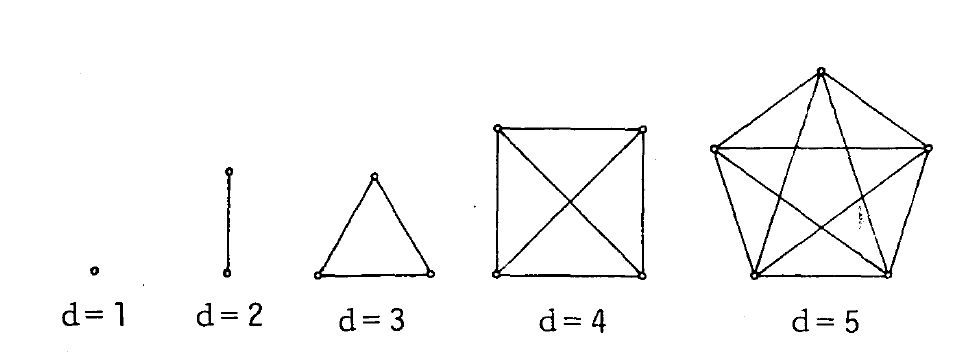
\includegraphics[width=1.00\textwidth]{images/ceyhun-011-fig01}
	\caption{Dolu çizgelere örnek.}
	\label{fig:doluCizgelereOrnek}
\end{figure}
\par \noindent
Dolu çizgeler için ayrıt sayısının,
   	 \[
		a = \tfrac{1}{2}d (d-1)
	\]
olacağı hemen görülecektir. Öyleyse, yalın çizgelerin ayrıt sayısı a,
	\[
        	0 \leq a \leq \tfrac{1}{2}d (d-1)
   	 \]
eşitsizliğini sağlayacaktır.
\end{document}